% arara: xelatex
% arara: xelatex
% arara: xelatex

% options:
% thesis=B bachelor's thesis
% thesis=M master's thesis
% czech thesis in Czech language
% english thesis in English language
% hidelinks remove colour boxes around hyperlinks

\documentclass[thesis=M,english]{FITthesis}[2012/10/20]

\usepackage[utf8]{inputenc}

\usepackage{graphicx} %graphics files inclusion
% \usepackage{subfig} %subfigures
% \usepackage{amsmath} %advanced maths
% \usepackage{amssymb} %additional math symbols

\usepackage{dirtree} %directory tree visualisation

% ADDED BY ME
\usepackage{blindtext} % lorem ipsum
\usepackage{todonotes} 

\newcommand{\todotext}[1]{\textcolor{red}{\textbf{[[#1]]}}}
\newcommand{\redtext}[1]{\textcolor{red}{[[#1]]}}
\definecolor{mygray}{gray}{0.6}
\newcommand{\blind}[1][1]{\textcolor{mygray}{\Blindtext[#1][1]}}

\setlength{\fboxsep}{0.005pt}
\newcommand{\tmpframe}[1]{\fbox{#1}}
%\renewcommand{\tmpframe}[1]{#1}

\let\myCite\cite
\renewcommand\cite{\unskip~\myCite}
\let\myRef\ref
\renewcommand\ref{\unskip~\myRef}

% \usepackage{spverbatim} % verb and verbatim with line breaks - doesn't break what I need

\newcommand\hatx{\^{}}



% list of acronyms
%\usepackage[acronym,nonumberlist,toc,numberedsection=autolabel,nomain]{glossaries}
\iflanguage{czech}{\renewcommand*{\acronymname}{Seznam pou{\v z}it{\' y}ch zkratek}}{}
%\makeglossaries

\newcommand{\tg}{\mathop{\mathrm{tg}}} %cesky tangens
\newcommand{\cotg}{\mathop{\mathrm{cotg}}} %cesky cotangens

% % % % % % % % % % % % % % % % % % % % % % % % % % % % % % % % % % % 
% % % % % % % % % % % % % % % % % % % % % % % % % % % % % % % % % % % 
\department{Department of theoretical computer science}
\title{Contextual Shell History}
\authorGN{Šimon} %author's given name/names
\authorFN{Let} %author's surname
\authorWithDegrees{Bc. Šimon Let} %author's name with academic degrees
\author{Šimon Let} %author's name without academic degrees
\supervisor{Ing. Lukáš Bařinka}

\acknowledgements{I would like to thank my supervisor Ing. Lukáš Bařinka for his guidance and advice. His insights and expertise shaped this work significantly. 

Next, my thanks goes to my colleagues and friends for their valuable feedback. They helped me spot my personal biases and assumptions rooted in my personal shell workflows. 

I am grateful for the trust of hundreds of people who downloaded this project. I would also like to thank all GitHub users who submitted issues and pull requests to the project.

I want to thank Installfest conference organizers for the opportunity to give a talk and to demo this project on Installfest.  

Finally, I would like to thank my family for their support during writing this thesis and trough my whole studies.
}
\abstractCS{\todotext{TODO: CZ abstrakt}  \blind[2]}
\abstractEN{\todotext{TODO: abstract} This thesis is an enhancement for standard shell history. It records shell history with context. It uses the recorded context to make it easier to find relevant history records and to make it possible to search search history using context explicitly.

\blind[2]
}
\placeForDeclarationOfAuthenticity{Prague} %where you have signed the declaration
\keywordsCS{Shell, Příkazová řádka, Historie shellu, Nástroje produktivity}
\keywordsEN{Shell, Command line, Shell history, Productivity tools}
\declarationOfAuthenticityOption{1} %select as appropriate, according to the desired license
% \website{https://github.com/curusarn/master-thesis} %optional URL (remove entirely if you have no URL for this thesis) TODO: put the thesis up

\begin{document}

%\newacronym{GUI}{GUI}{Graphical User Interface}
%\newacronym{CLI}{CLI}{Command Line Interface}
%\newacronym{GNU}{GNU}{GNU's Not Unix!}
\begin{introduction}



Classic command line interfaces were mostly replaced by GUIs in consumer software \cite{norman2007ui}. \todo{REF?} However, many professionals around the world still rely on UNIX shells to achieve their daily tasks. CLIs are generally not replaceable by GUIs because GUIs do not scale well when the number of available actions is high \cite{norman2007ui}. 

More than half of all developers use Unix-based operating systems\footnote{According to \cite{stackoverflow2019devsurvey}, 25.6\% and 26.8\% of developers uses Linux and MacOS respectively.}. 
About half of all developers have been working with Linux during year 2018. \cite{stackoverflow2019devsurvey} 

Default shell on GNU/Linux is Bash \cite{ramey1994gnubash} and default shell on MacOS is zsh since October 2019 \cite{apple2019zsh}. In this work we primarily focus on these two popular shells.
\todo{TODO: polish the argument why is this work relevant \hatx\hatx\hatx}

\todotext{TODO: what is the shell history good for}
\todotext{TODO: why could contextual history improve the history offerings}

The standard shell history contains records with basic information about previously executed command lines. Each record only contains following details: the command line, timedate of the execution, and the duration of the execution\footnote{Duration is only available in Zsh and only when it is enabled.\cite{zshdocs}}. 

Additionally, it is quite common to use shell configuration\footnote{\todotext{e.g. Bash: histocontrol=ignoredups\cite{bashman}; zsh: HIST\_SAVE\_NO\_DUPS\cite{zshdocs}}} to prune duplicates from the history. This removes more information from history because the original command line sequences are lost.

As we can see the standard shell history contains only very basic information about executed command lines.
There is much more contextual data available at the time of command line execution e.g. present working directory, exit status, and previously executed commands. In this work, we explore the possibilities of using the contextual data about executed commands to increase the usefulness of shell history.



% BAD: This limits the potential of standard shell history utilities because shell usage is contextual. is not generally used to run ad-hoc commands but 

% MORE PRACTICAL: When using shells you likely do not run individual commands completely independently of each other. But instead run commands as parts of different workflows that 

\todo{describe the contents of this work / layout - redo because moved chapters in analysis} We start by analysing shell history features to understand advantages and disadvantages of standard shell history. We research existing history tools to see what ideas were already explored, which features work and which do not. 

After that, we focus on people. We start broad and research how people use computer tools in general. Then we move on to examining how people use shell and shell history. We also look at public discourse related to history tools and engage in online discussions to find out more about configurations and tools people use.

Next, we focus on the contextual information; We cover what information is available to be saved at the time of command line execution and we discuss how it could be used to enhance shell history. 

At this point we move on to design(ing) ...
\todotext{TODO: finish this intro}


\blind[2]

\end{introduction}


\chapter{Analysis}

\todo{DEFINE "command line entry"/"history entry" is a full command entered/submitted by the user}
\todo{DEFINE "stub" is the first word of the command line entry - usually an executable, a shell builtin, or an alias.}

\todo{REPLACE "command line" -$>$ "command line entry"}
\todo{REPLACE "command" -$>$ "stub"}

\todotext{TODO: describe layout/contents of the chapter}

\blind

\section{Origins of standard history features in shells}

In this chapter we explore the standard shell history features which are most likely available to majority our target users.
Most of the history features we see and use today were adopted from older shells. Many of these features stayed similar to their original versions. We look at the shells and the history features chronologically to see the evolution and improvements in shell history facilities over the years.  


\begin{figure}
  \tmpframe{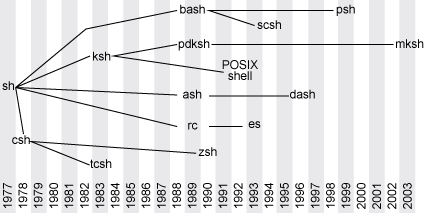
\includegraphics[width=\linewidth]{figures/misc/shells.png}}
  \caption{Linux shells since 1977, from \cite{jones2011shells} \todotext{TODO: Better quality or begone.}}
\end{figure}

\todotext{TODO: Add summaries of the features using bullet point lists.}
\todotext{TODO: Point out drawback of the features as you describe them.}
\todotext{TODO: Break up the walls of text with bold text and bullet point lists.}

\subsection{History features of C shell}

C shell (Csh) was initially released in 1978. 
It features history substitution: a simple history mechanism enabling reuse of previously executed commands inspired by Interlisp\cite{joy1994cshintroduction}. Size of the history is configurable\footnote{Examples featured in \cite{joy1994cshintroduction} and \cite{dubois1995tcshusing}
show history size set to 10 and 20 records respectively.} but according to \cite{cshman}, too large values may run the shell out of memory.

% History is disabled by default (I think) persistence accross sessions is on my install

C shell history substitution allows the user to reuse: the previous command line using \verb|!!|, the last argument of the previous command line using \verb|!$|, and all arguments of the previous command line using \verb|!*|. To run other commands lines than the previous one we could use \verb|!cc| which executes the last command line from history starting with \verb|cc|. Executing a command line based on absolute or relative index can be done using \verb|!5| or \verb|!-2| respectively. To see what command is about to be executed we could use e.g. \verb|!cc:p|, \verb|!5:p|, or \verb|!-2:p|; This only prints the history record instead of executing it. It is also possible to replace parts of command lines using \verb|!!:s/foo/bar/| or a shorthand \verb|^foo^bar| where \verb|foo| is replaced by \verb|bar| in the previous command and the result gets executed. \redtext{When using these features we do not see the resulting substituted command line until executing it. This can lead to errors or printing the substitutions first which slows users down.}
    
There is a \verb|history| command which prints out recent history records with their indexes. There are also other less notable history substitution features available; These are accessible using different modifiers that can follow \verb|!| character. Another noteworthy features of Csh are: file name tab completion, tilde expansion, command aliases, and job control.\todo{check \& ref? } \redtext{history can be easily persisted across logins}

\redtext{savehist - allows to merge history instead of overwriting it}
%savehist
%If set, the shell does 'history -S' before exiting. If the first word is set to a number, at most that many lines are saved. (The number must be less than or equal to history.) If the second word is set to 'merge', the history list is merged with the existing history file instead of replacing it (if there is one) and sorted by time stamp and the most recent events are retained. (+)
\redtext{commands lines are saved to history after the history expansion is performed}


\subsection{History features of Tenex C shell}
Tenex C shell (Tcsh) is an enhanced version of the C shell released in 1983\todo{REF}; It offers command line editing and programmable tab completion\cite{dubois1995tcshusing}. Since Tcsh is a version of C shell, it does support all the previously described features of C shell. The history holds 100 previous command lines by default and it also contains datetime of the command line execution.


Tcsh offers command line editing; This means that the user can manipulate the contents of the command line by using various built-in functions. A few examples of such functions are: \verb|delete-word|, \verb|expand-glob|, and \verb|history-search-backward|. All built-in functions can be bound to arbitrary key combinations. Additionally, Tcsh features emacs and vi editing modes which come with default keybindings usual for the respective editors. When describing the default keybindings for Tcsh in this section we are only considering the emacs mode.

A portion of built-in functions allows the user to reuse command lines from the shell history. Functions \verb|up-history| and \verb|down-history| allow the user to step through the history; Default keybindings are \verb|CTRL-P| and \verb|arrow_up| for \verb|up-history|; and \verb|CTRL-N| and \verb|arrow_down| for  \verb|down-history| \cite{tcshman}. This is something you are likely already used to in your modern shell.

  
% BAD ALT: Pressing \verb|CTRL-P| invokes \verb|up-history| function which replaces the current command line contents with previous command line from history. Pressing \verb|CTRL-P| repeatedly continues up through the history. Pressing \verb|CTRL-N| invokes \verb|down-history| function which steps through the history in the other direction. These two functions are also often bound to \verb|arrow_up| and \verb|arrow_down| keys. 

Besides stepping through history, Tcsh features prefix search. The functions \verb|history-search-backward| \todo{make sure this doesn't overflow :( } and \verb|history-search-forward| use the command line contents before the cursor as a prefix to search the history in the desired direction. The default keybindings for these functions are a little weird; \todo{TODO: Pressing ESC an then x is just a way of pressing ALT-x without having ALT. }
You need to press \verb|ESC| and then \verb|p| or \verb|n| for backward or forward search respectively. 

Another useful history feature of Tcsh is interactive string search. In contrast to prefix search this feature allows us to search history using any part of the command line not just the prefix. This feature is realised by \verb|i-search-back| and \verb|i-search-fwd| functions. Invoking these functions prints a secondary prompt under the primary one: \verb|bck:| or \verb|fwd:| depending on the invoked function. Typing searches the history interactively in the desired direction. Invoking the functions repeatedly steps through the history records that match the query.
These functions sound quite useful but despite that they are not bound to any keys by default.
% \redtext{So the users need to set up the key bindings themselves.}

Activating vi mode in Tcsh changes some of the keybindings. In addition to regular keybindings, stepping through history is available on keys \verb|K| and \verb|J|, and prefix search is available on \verb|SHIFT-K| and \verb|SHIFT-J|. Instead of \verb|i-search-back| and \verb|i-search-fwd| functions vi mode offers \verb|vi-search-back| and \verb|vi-search-fwd| with similar functionality.
% \redtext{vi mode has defaults - back: ? ,fwd: /}

\redtext{histdup - prunes duplicates from history}
% tcsh man page (+ means "not available in csh")
%histdup (+)
%               Controls  handling  of  duplicate  entries in the history list.  If set to `all' only unique history events are entered in the history list.  If set to `prev' and the last
%               history event is the same as the current command, then the current command is not entered in the history.  If set to `erase' and the same event is  found  in  the  history
%               list, that old event gets erased and the current one gets inserted.  Note that the `prev' and `all' options renumber history events so there are no gaps.


% Since we are mainly interested in history features we only focus on the functions that use history 
% Command line editing was an important step forward in interactive shell use. It enables the user
% As the name suggest it was inspired by features available in Tenex operating system. 

\subsection{History features of Korn shell}
Korn shell (Ksh) was initially released in 1983; It was originally written as a proprietary software until being released as open source in 2005. \todo{REF} History features of Korn shell are a very similar to the features of Tenex C shell. Ksh offers stepping through history, string search, and vi mode variant of the string search. It is worth mentioning that in Ksh, string search is bound to \verb|CTRL-R| by default which is what you are probably used to in modern shells. 

Ksh offers a shell builtin command \verb|fc| that provides a superset of C shell history mechanism\cite{rosenblatt2000kshlearning}. It allows the user to list recent history entries, edit command lines from history with an editor, and run history entries with changes. Running \verb|fc -l| lists the previous command lines from history (with indexes). So does \verb|history|, because in Ksh it is just an alias for \verb|fc -l|. To edit previous command line from history in an editor we could use \verb|fc| (without arguments) which executes the resulting command after we are done editing it. If we want to choose an editor we could use \verb|fc -e vi|. Running \verb|fc -e - foo=bar| skips the editing, replaces occurrences of \verb|foo| with \verb|bar| and executes the result. To access more then the previous command line we would use absolute or relative indexes similarly to the history expansion in Csh. For example, \verb|fc 5| and \verb|fc -2| opens an editor with fifth from the history list and the second command relative to current command line. It is also possible to select ranges of commands for editing with e.g. \verb|fc -2 -6|.

% We are not describing other Ksh history features in detail because of the similarity with already described Tcsh history features.


\subsection{History features of Bourne again shell}
Bourne again shell (Bash) was initially released in 1989.
Default history size in Bash is 500 records.\cite{bashman} Each history entry contains datetime of the execution. Unless the user disables the \verb|cmdhist| option, all lines of a multi-line command are saved as one history record; Based on \verb|lithist| option, newlines are either embeded into history or replaced by semicolons to keep the syntax of the saved commands correct. 

There are shell variables that can be used to prevent certain command lines from being saved to history. Variable \verb|HISTCONTROL| can be used to prevent saving duplicates, and to skip saving command lines starting with a space. Variable \verb|HISTIGNORE| allows using pattern matching to prevent various command lines from being saved into history.  

Bash features history expansion (\verb|!!|, \verb|!$|, \verb|!cc|, etc.) which is compatible with the Csh\cite{ramey1994gnubash}.
Bash features a \verb|histverify| option that alters the behaviour of history expansion. When it is enabled, the results of history expansion are  pasted onto the command line instead of being executed immediately. This option is disabled by default. 

\todo{COMMENTED: use this later as an example for memory load}
% It seems that authors of Bash realised the danger of history expansion; It forced the users were either forced to rely on their memory or to explicitly ask for the history expansion result to be printed first.}
% This shows us both the importance of not relying on memory/recall and the importance of adhering to the existing standard.
\todo{NOTE: we could briefly introduce Readline}
Command line editing in Bash provides most of the history related functions from Tcsh. Some of these functions have different names and some of them have different default keybindings.

Functions for stepping through history \verb|up-history| and \verb|down-history| are named \verb|previous-history| and \verb|next-history| respectively; Default keybindings did not change. 

Interactive string search (better known as reverse search) is available in Bash as \verb|reverse-search-history| and \verb|forward-search-history| with default keybindings \verb|CTRL-R| and \verb|CTRL-S|. 
Common issue with this keybinding is that \verb|CTRL-S| is often used to freeze the output of the terminal using OS's terminal driver\todo{REF: ask Barinka, he will know}; This means that many users do not have the option to search in the "forward" direction.   
Bash also provides non-interactive versions of these functions bound to \verb|ALT-P| and \verb|ALT-N|. However, besides saving your CPU from searching the history multiple time, they do not seem to provide any advantage over their interactive counterparts. 

Prefix search functions are still available under the same name (\verb|history-search-backward| \todo{overflow!} and \verb|history-search-forward|) but they do not have default keybindings in Bash. Alternative substring searching versions for these functions are available which do not search just by prefix but can match anywhere on the command line: \verb|history-substring-search-backward| and \verb|history-substring-search-forward|.\todo{overflow!}

Another two history functions we can find in Bash are \verb|yank-last-arg| and \verb|yank-nth-arg|. The first one pastes the last argument of the previous history entry onto the command line. The second one pastes the Nth argument. Default keybindings for \verb|yank-last-arg| are \verb|ALT-.| or \verb|ALT-_|. To use \verb|yank-nth-arg| we need to provide an argument to Bash input library; This can be done by pressing an \verb|ALT| key with a numeric argument. Then we can press \verb|CTRL-ALT-Y|. Without providing any argument the function pastes the first argument of the previous history entry onto the command line.


Other than command line editing functions Bash offers builtin commands to list, reuse and manipulate the history. The \verb|fc| builtin is very similar to the one available in Ksh. We can list of recent command lines from history with \verb|fc -l|, edit and execute them with \verb|fc| without any arguments, and substitute and execute them with \verb|fc -s foo=bar|. It is possible to select command lines and ranges of command lines from the history using absolute or relative indexes.

Compared to Ksh, \verb|history| is no longer just an alias; It is a Bash builtin which can be used to display and control the shell history. Without any arguments, \verb|history| prints out a list of previous history entries with indexes. Using various command line options it can be used to: add command lines to history, delete them, or clear the history. It can load new or all history entries from the history file to the history of this shell session; New entries could appear in the history file because of other simultaneously running shell sessions. Conversely, we can use the \verb|history| builtin to append or write the history of this shell session to the history file.


\subsection{History features of Z shell}

Z shell (Zsh) was originally released in 1990. Most of the history features available in Bash are also offered by Zsh.
The default history size is just 30 lines. The history contains the executed command line, the datetime and the duration of the execution. This information is only saved to history when the \verb|EXTENDED_HISTORY| option is enabled. 

% Zsh is overall more feature-rich than Bash. 
% Many features and options that are natively supported in Zsh are non-trivial or impossible to set up in Bash\todo{example?, ref?}.
% We are not going to cover Zsh in great detail because of its similarity to Bash.

Zsh does feature csh-style history expansion. Like Bash, it can be configured to evaluate the history expansion and paste the result onto the command line instead of executing it; This behavior can be enabled using \verb|HIST_VERIFY| option. Another way to see what the history expansion evaluates to is the \verb|magic-space| function. It evaluates history expansion and inserts a space when invoked. When we bind this function to spacebar the history expansion will get evaluated every time we press \verb|SPACE|.

\todo{NOTE: we could briefly introduce ZSH ZLE}
We can find Zsh equivalents for almost all Bash command line editing functions that allow history reuse. In addition, we can find variations and extra functions compared to what is available in Bash. Using \verb|arrow_up| and \verb|arrow_down| keys we can retrieve recent command lines from history. Prefix search is available but unbound by default. There is a variant of prefix search that always searches by first word on the current command line no matter where the cursor is. This variant of prefix search is bound to \verb|ALT-P| and \verb|ALT-N| by default. Interactive reverse search functions are also available with the same default keybindings as in Bash.

Zsh offers pattern matching variants for the most of the history searching functions; These treat the typed query as a pattern instead of a string that should be matched exactly. Vi mode variants for some of the searching functions are available as well.  

The \verb|fc| builtin command is supported and the functionality is comparable to its Bash counterpart. Like in Ksh, \verb|history| is just an alias for \verb|fc -l|. 

% There are alternatives to achieve almost anything that can be done in Bash. For example, ...


\blind
\todotext{TODO: short conclusion about shells ? }


\section{How people use shell}

In this chapter we examine how people use shell and shell history. We consider previous research that studies the properties of how people use command based systems. We also collected a sample of user shell histories and we will be discussing where our data matches the existing findings and where it does not. 

We are looking at properties of command line usage to see if find justifications for standard history features. Examining shell history could also give us insights into how to design history tools. 

After examining shell usage itself we focus on how people use shell history features. We explore existing online discourse about history tools to discover common workflows, problems and configurations.

\subsection{Collecting shell history}

\todotext{TODO: describe how we collected history (skipping errors)}
\blind

\subsection{Frequency distributions of commands}

In this section, we focus on commands instead of whole command lines. By command we mean the first word of the command line executed by the user. Command is usually an executable program or a shell builtin.

\redtext{According to \cite{greenberg1993computer}, frequency distribution of commands used by a group of similar users follows Zipf distribution.}

\redtext{Zipf distribution has the property that a relatively small number of items have high usage frequencies, and a very large number of items have low usage frequencies.}

\todotext{TODO: 80-20 rule is a looser characteristic of Zipf distribution - 20 \% of items account for 80 \% of usage ... alternative 90-10}
\blind
80-20 rule -$>$ https://en.wikipedia.org/wiki/Pareto\_principle



\todotext{TODO: describe and explain the plots}

% A looser characteristic of this kind of rank distribution is the well-known 80-20 rule of thumb that has been commonly observed in commercial transaction systems - 20\% of the items in question are used 80\% of the time (Knuth, 1973; Peachey,Bunt, and Colbourn, 1982).2

% In measurements recorded from a UNIX site, Hanson, Kraut, and Farber (1984) report a similar trend - 10\% of the 400-500 commands available account for 90\% of the usage


% Figure 3.1. The normalized command frequency, compared with Zipf.

\begin{figure}
  \tmpframe{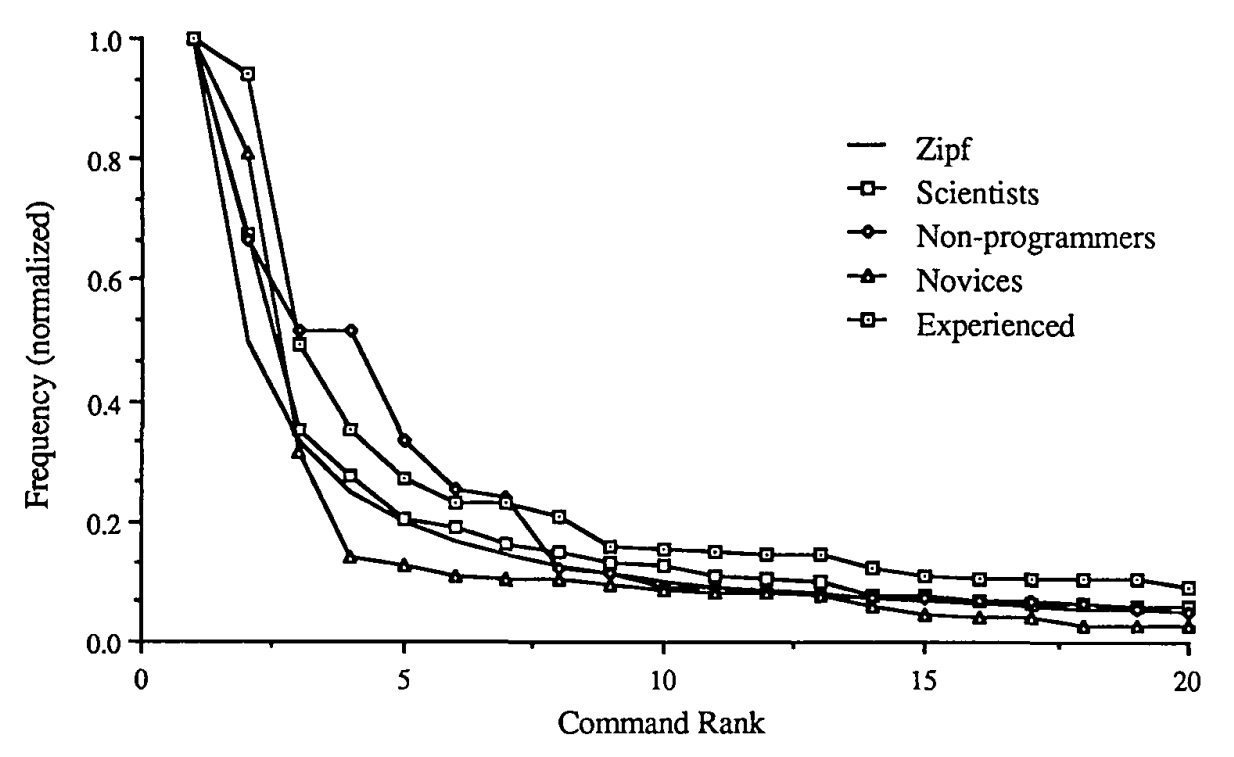
\includegraphics[width=\linewidth]{figures/greenberg/plot_ref_zipf-cmd-frq.png}}
  \caption{The normalized command frequency, compared with Zipf from \cite{greenberg1993computer}}
\end{figure}

\begin{figure}
  \tmpframe{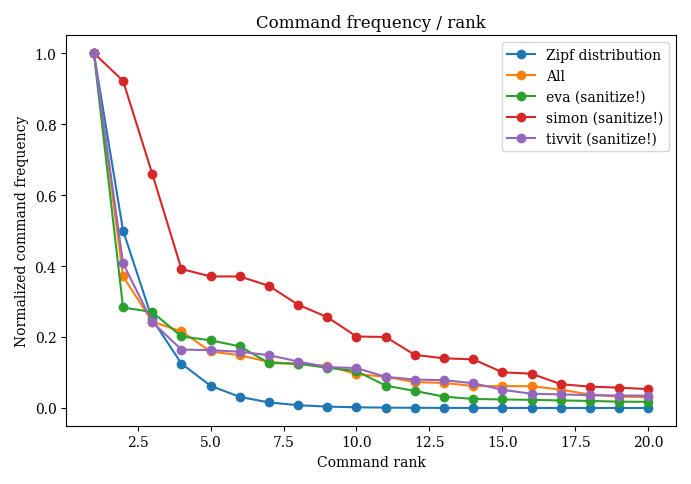
\includegraphics[width=\linewidth]{figures/greenberg_new/plot_zipf-cmd-frq.png}}
  \caption{The normalized command frequency, compared with Zipf. \todotext{unify labels to match Greenberg, export in vector, lose top title, add data from more people}}
\end{figure}
\todo{command rank plots should be on the same page}
\todo{make sure figures are not all over the place}

\todotext{TODO: In our plot the combined history of all the subjects somewhat follows zipf. BUT also most of the individual users follow the zipf - there are exceptions. In Greenberg study individual histories did not follow zipf.}

% ALL: Top 100 %% of cmds amounts for 100.0 %% of all command lines
% ALL: Top 10 %% of cmds amounts for 63.43728659230594 %% of all command lines
% ALL: Top 20 %% of cmds amounts for 71.34987480081949 %% of all command lines
% eva: Top 100 %% of cmds amounts for 100.0 %% of all command lines
% eva: Top 10 %% of cmds amounts for 62.012411347517734 %% of all command lines
% eva: Top 20 %% of cmds amounts for 73.35992907801419 %% of all command lines
% simon: Top 100 %% of cmds amounts for 100.0 %% of all command lines
% simon: Top 10 %% of cmds amounts for 57.7319587628866 %% of all command lines
% simon: Top 20 %% of cmds amounts for 66.18556701030928 %% of all command lines
% tivvit: Top 100 %% of cmds amounts for 100.0 %% of all command lines
% tivvit: Top 10 %% of cmds amounts for 53.33086145099493 %% of all command lines
% tivvit: Top 20 %% of cmds amounts for 64.93634902978619 %% of all command lines


\todotext{TODO: According to \cite{greenberg1993computer},: For each of the four
user groups, 10\% of the commands used accounted for 84\%-91\% of all usage}


\redtext{Top 10 \% of cmds amounts for 63 \% of all command lines}
\redtext{Top 20 \% of cmds amounts for 71 \% of all command lines}

\redtext{Our data does somewhat follow the 80-20 (71-20) rule (relatively few items account for a significant portion of the distribution) but it is a significant difference compared to the stats from the study. Because of the low number of subjects we can only theoretize why this is - more commands available?, small sample size?, longer collection period?}

\redtext{We suspect that difference is mainly caused by larger number of commands used by the users overall}

\redtext{TODO: Top used commands differ between people}
\redtext{According to greenberg, even when people have very similar expertise and identical goals the commands they use vary significantly. Surprising number of commands is not shared by the users from the same group. This diversion shows that there are many ways to achieve the same goal. Commands are smaller units that make up the goals of the users. - Our data is in line with these ideas.} 

\todotext{Conclusion: Command frequencies are highly uneven and individual.}

\subsection{Command Vocabulary}

\redtext{Command vocabulary is the set of commands used by a given person. We are interested in analysing how the vocabulary of the user changes over time.}

\todotext{TODO: describe and explain plots}


% Figure 3.2. Command vocabulary size vs. the number of command lines entered for four individuals.

\begin{figure}
\centering
  \tmpframe{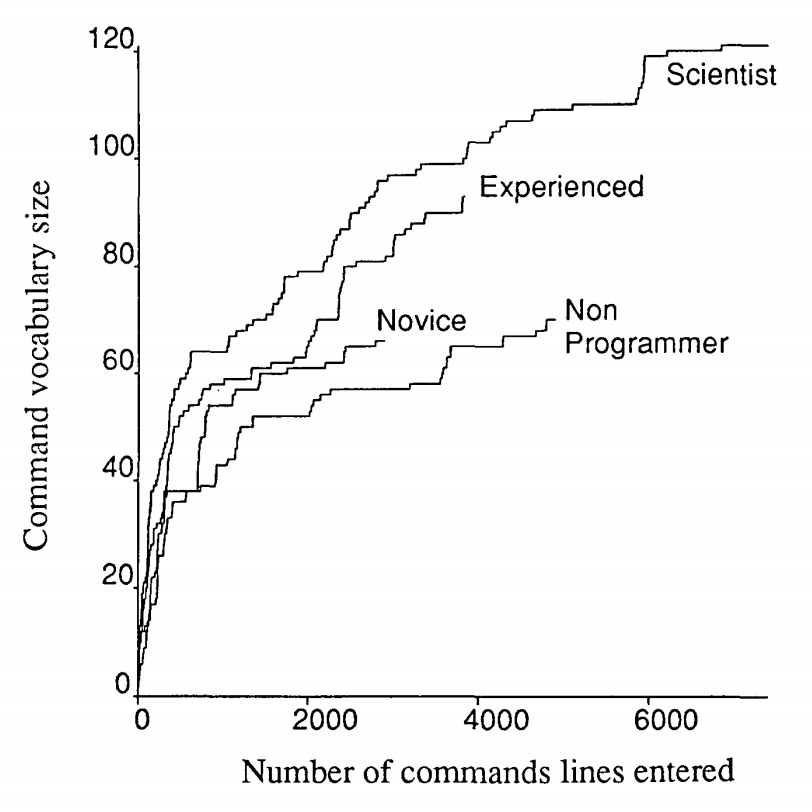
\includegraphics[width=0.6\linewidth]{figures/greenberg/plot_ref_cmd-vocab-size.png}}
  \caption{Command vocabulary size vs. the number of command
lines entered for four individuals. (Greenberg)}
\end{figure}

\begin{figure}
  \tmpframe{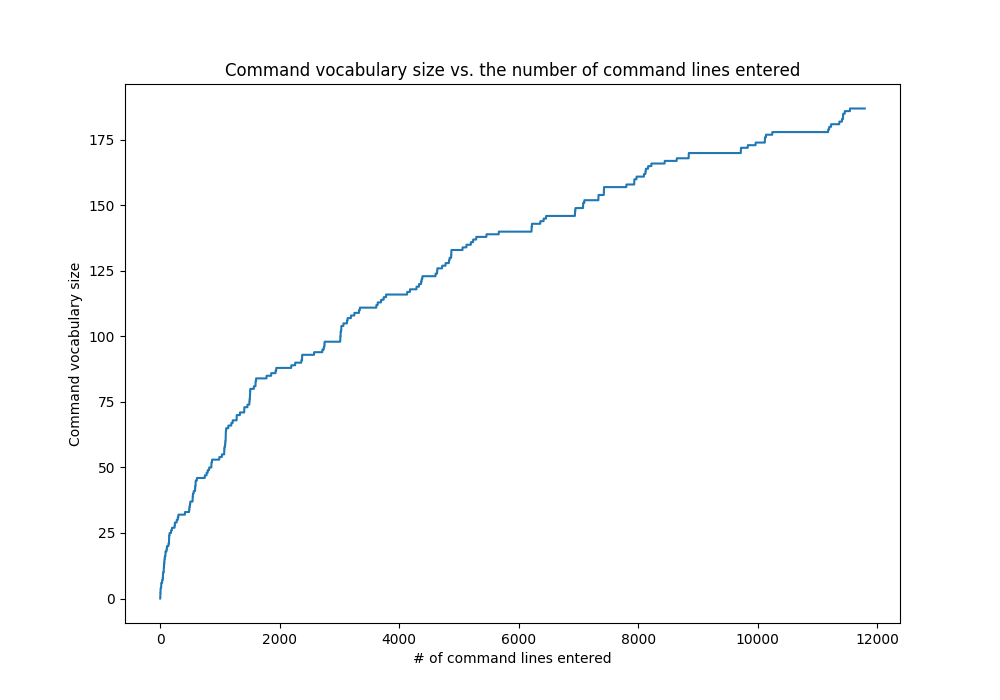
\includegraphics[width=\linewidth]{figures/greenberg_new/plot_cmd-vocab-size.png}}
  \caption{Command vocabulary size vs. the number of command
lines entered for \todotext{N individuals}}
\end{figure}

\begin{figure}
  \tmpframe{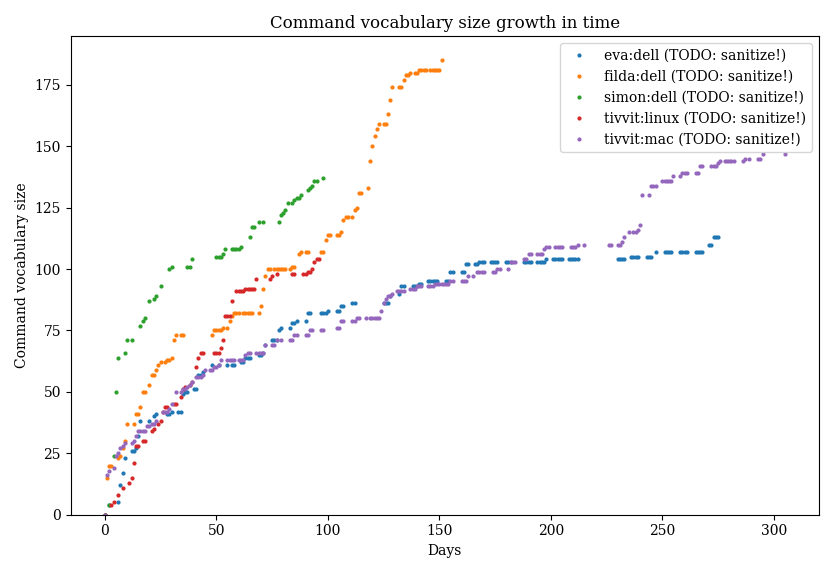
\includegraphics[width=\linewidth]{figures/greenberg_new/plot_cmd-vocab-size-time.png}}
  \caption{Command vocabulary size in time of \todotext{N individuals} (empty spaces are for days without any shell history)}
\end{figure}




\todotext{TODO: initial "steep" period in the plot is caused by the system encountering the commands for the first time. the more stable part is more representative of actual adoption rate of new commands.}

\todotext{TODO: Greenberg found out that bursts in adoption of new commands is sometimes caused by new goals of the user but sometimes no such new goal can be found in the data. Our data does support this. }

\redtext{Greenberg reports adoption or about 5\% for all users before they enter 1k command line. He concludes that this is an initial learning period when the system encounters most of the commands for the first time. According to Greenbers, after initial 1k cmd lines entered the adoption rate drops quicky under 1\%. This is somewhat in line with our findings. We did observe about 5\% cmd adoption rate during the first 1k cmdlines entered for vast majority of our users. Between 1k and 2k we saw a drop in adoption of new commands to about 3\%. After 2k the adoption dropped to numbers lower than 2\% for most users.}

\todotext{TODO: Two differences - longer initial period of 2k cmdlines and higher adoption rate of up to 2\%}

\redtext{These differences could be caused by multiple factors. There is more commands available compared to XX years before. Additionally, custom commands/scripts seem to be quite common in our data while they seem to be non-existent in the greenberg study. This alone could have a huge impact. Draper (see below) was referring to a number of commands available to users of ... as 570. }

\redtext{Nowadays the number of available commands is virtually unlimited because users can install and create new commands. Number of initially available commands on a newly installed system is in thousands.}

% REF: Draper (1984) estimated the times a command was invoked by noting the UNIX processes spawned during each user's interaction with the system (method 4, Section 2.2.1).5 He suggested that the overall trends observed are representative of real command use. First, out of a vocabulary of the 570 commands available to the population, only 394 (70\%) were used at least once. 

\redtext{We can conclude that command usage distribution was and still is very uneven (few commands dominate the distribution) and that the number of available commands slowly and unevenly increases over time but the adoption of new commands is faster than in the past.}

\redtext{new workflows, aliases, ...}

% eva: Cmd adoption rate at 1k (between 0 and 1k) cmdlines = 0.051
% eva: Cmd adoption rate at 2k cmdlines = 0.0345
% eva: Cmd adoption rate between 1k and 2k cmdlines = 0.018
% eva: Cmd adoption rate between 2k and 3k cmdlines = 0.013
% eva: New cmd adoption rate after 1k cmdlines = 0.007725856697819315
% eva: New cmd adoption rate after 2k cmdlines = 0.006263345195729538
% eva: New cmd adoption rate after 3k cmdlines = 0.005145228215767635
% simon: Cmd adoption rate at 1k (between 0 and 1k) cmdlines = 0.076
% simon: Cmd adoption rate at 2k cmdlines = 0.0505
% simon: Cmd adoption rate between 1k and 2k cmdlines = 0.025
% simon: Cmd adoption rate between 2k and 3k cmdlines = 0.007
% simon: New cmd adoption rate after 1k cmdlines = 0.015840041547649963
% simon: New cmd adoption rate after 2k cmdlines = 0.012627148368993335
% simon: New cmd adoption rate after 3k cmdlines = 0.015667206915180983
% tivvit: Cmd adoption rate at 1k (between 0 and 1k) cmdlines = 0.045
% tivvit: Cmd adoption rate at 2k cmdlines = 0.0315
% tivvit: Cmd adoption rate between 1k and 2k cmdlines = 0.018
% tivvit: Cmd adoption rate between 2k and 3k cmdlines = 0.011
% tivvit: New cmd adoption rate after 1k cmdlines = 0.009304948540814888
% tivvit: New cmd adoption rate after 2k cmdlines = 0.007877892663712457
% tivvit: New cmd adoption rate after 3k cmdlines = 0.007264873355586099
% >>> Avg recurrence rate = 70.29523637022278
% >>> Max avg recalled characters = 16.34658576344865
% >>> Max avg recalled characters (including prefix matches) = 26.770874841514217

\subsection{Sequential dependencies between commands}

We just looked at frequencies of commands and command vocabulary of shell users. Now we take a look the dependencies between commands.

\todotext{TODO: describe the graph by Hanson - all users together, node size indicates frequency of the command, arrows indicate significant dependencies, 50 cmds. }

\todotext{TODO: describe findings by Hanson - significant chains, core/modular cmds vs. cmds with significant dependencies, functional clusters of commands}



% Figure 3.3. Sequential structure of UNIX command usage, from Figure 4 in Hanson et al. (1984).

\begin{figure}
  \tmpframe{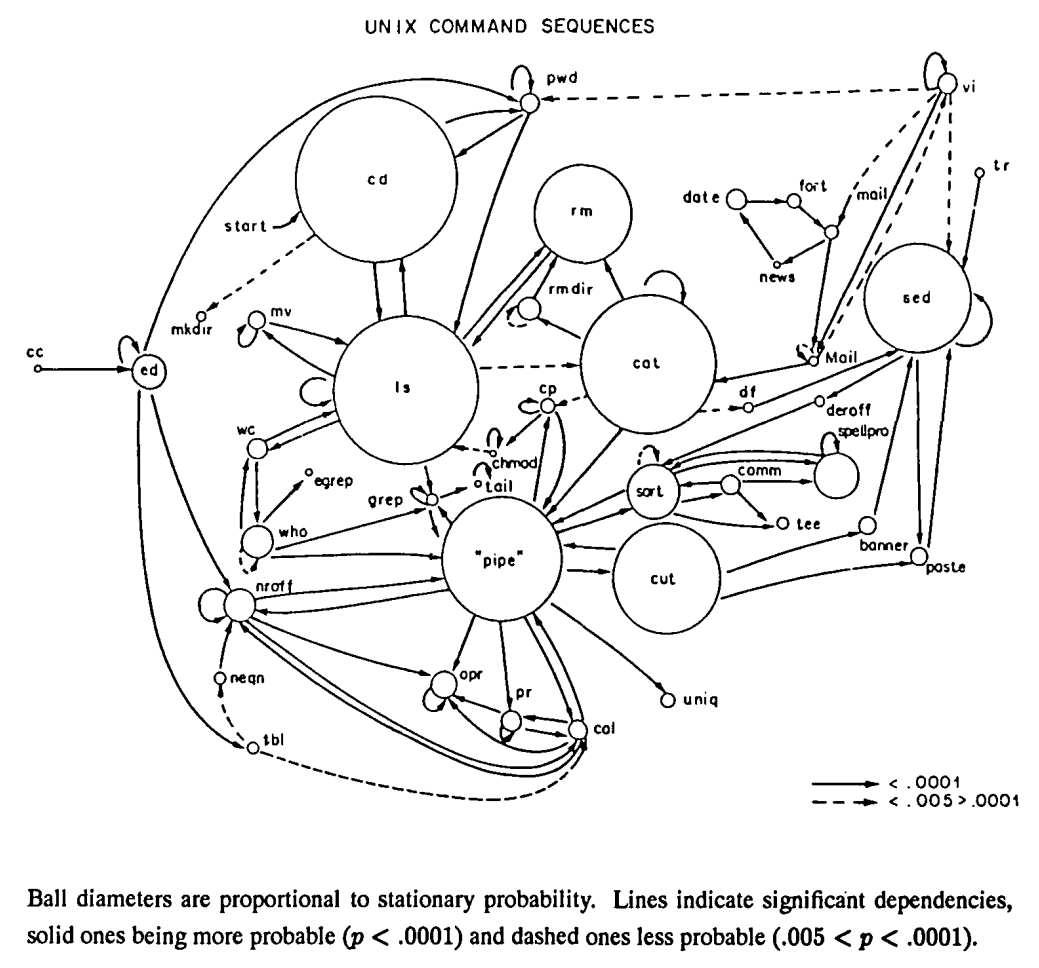
\includegraphics[width=\linewidth]{figures/greenberg/graph_ref_cmd-sequences.png}}
  \caption{Sequential structure of UNIX command usage, from Figure 4
in Hanson et al. (1984). (Greenberg)}
\end{figure}

\begin{figure}
  \tmpframe{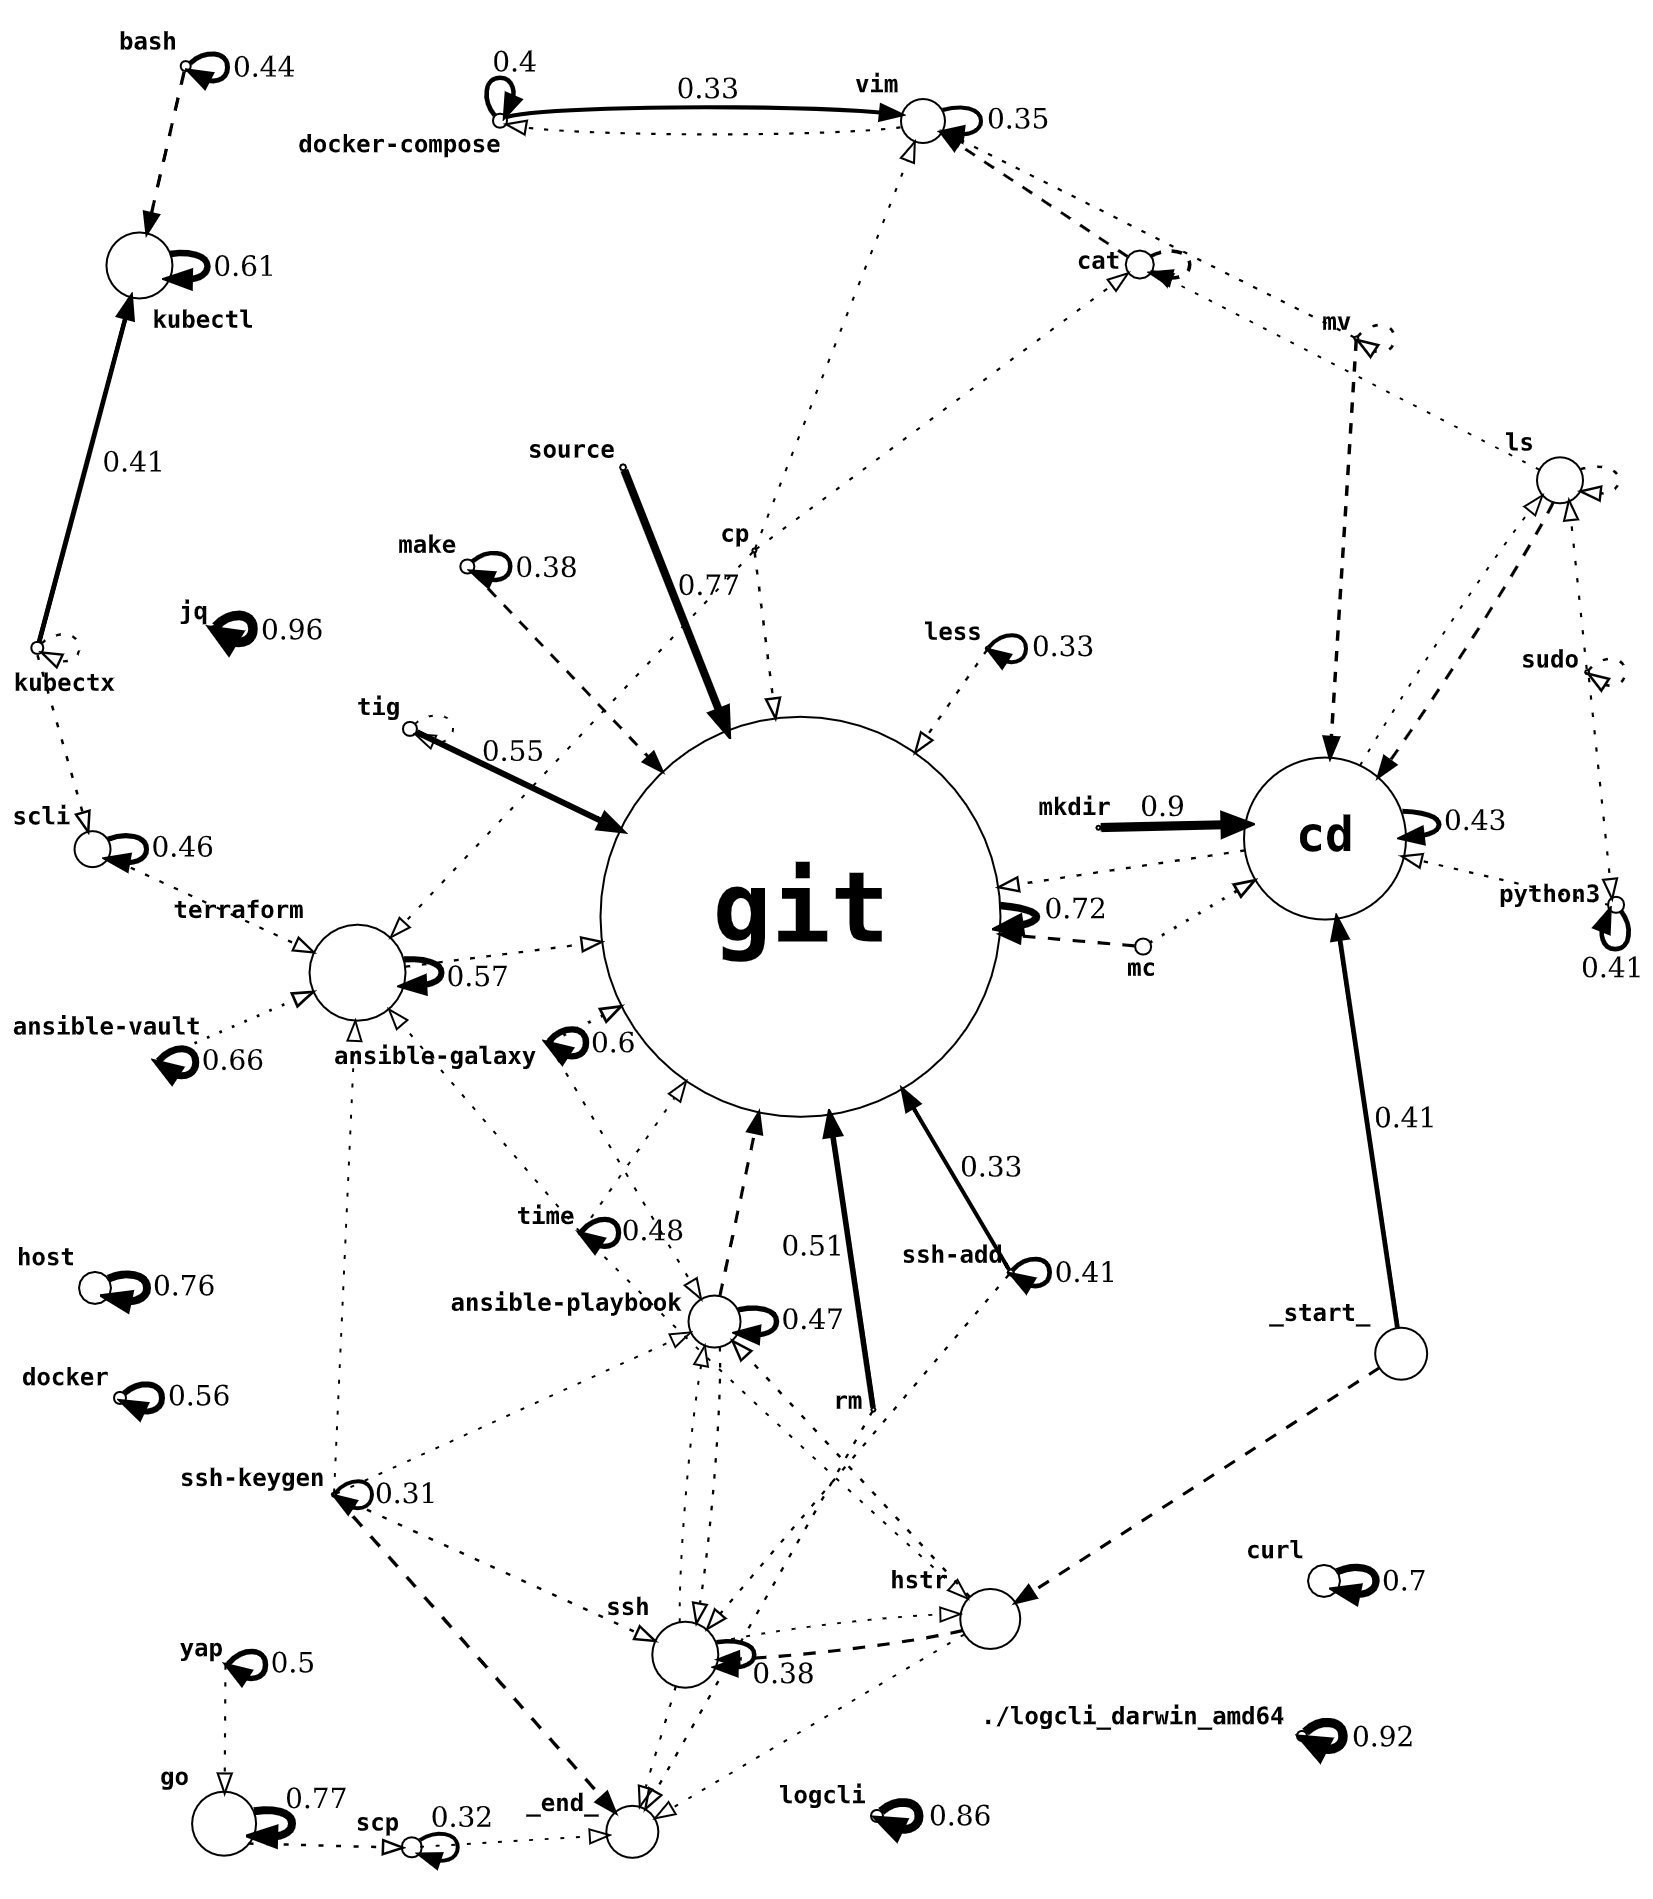
\includegraphics[width=\linewidth]{figures/greenberg_new/graph_cmd-sequence_vit_41_0-1_crop.png}}
  \caption{Sequential structure of command usage.}
  \label{seq-graph}
\end{figure}

\begin{figure}

\centering
\begin{tabular}{|l|l|}
\hline
Edge style & Transition probability            \\\hline
Regular/full     & 1.0 -- 0.3 (specified by labels) \\
Dashed      & 0.3 -- 0.2                         \\
Dotted      & 0.2 -- 0.1                         \\
\hline
\end{tabular}
\caption{Sequential structure of command usage (legend).}
\label{tab:seq-table}
\end{figure}

\todo{sequential graph and its legend table must be on the same page!}




% REF: "Through a multivariate analysis of UNIX commands invoked by the site population, Hanson, Kraut, and Farber (1984) examined the interaction effects between commands. Their results show statistically significant relationships between certain command chains; the relations between the fifty most frequently used commands are shown in Figure 3.3. Each ball in the network represents a command, its size indicates the usage frequency, and the arrow indicates the significant dependencies. One dimension of these relationships is modularity. Some commands, such as Is, are core commands - they are used frequently and are surrounded by many other commands (i.e., highly modular and independent). Others are not; they are surrounded by specific command sequences. An example of the latter is cp, which is generally preceded by itself and followed by chmod." "Commands are also related by functional clusters, such as editing, process management, orientation, social communication, and so on (Hanson, Kraut, and Farber, 1984), which may not be revealed by statistics."

\redtext{Greenberg concluded that assuming that the sequential dependencies of commands found by polling all the users together is a mistake.}

In earlier chapter, we saw that there are a big differences in vocabularies of different people so it is not surprising that sequential properties of the commands also differ significantly between individuals.

We created a graph sequential dependencies between commands for a selected individual. Since we are studying sequential properties of commands with the relation to history tools; We chose not to use the same method as Hanson so the graphs are not comparable. 

\todotext{TODO: polish this up}
We created the graph by taking 41 most used commands. Each node represents a command and the size of the node is proportionate to the command frequency. Each vertex represents a transition probability from one command to the next one. We decided to create the graph this way because it represents properties that could be potentially used in history tools; It only uses the probability of transition from one command to the next one. Hanson used a method which also considers the reverse transition probabilities; That is the probability that given command was preceded by the previous command. For example, when predicting the next command we only have the information about the past and current command. 


The \verb|_start_| command represents a start of a new terminal session.
The \verb|_end_| command represents an end of the terminal session; It does not matter how the session ended.

\todotext{Errors filtered out because we want to study the history to help people achieve their goals - filtering exit status !0 is not fully correct but the resulting data is more useful than without any filtering.}

\todotext{There are strong dependencies between certain commands - e.g. mkdir almost always followed cd - cd into the newly created directory, source is almost always followed by git w/o clear reason; Existence of strong dependencies suggests that it could be worth to predict the next command using the previous one.}

\todotext{Many commands have a high probability of being repeated - e.g. jq which is almost always followed by itself, curl, git, ssh ...; High rate of commands being repeated shows the need to recall recent history records - even the most immediate ones. Remember that these high rates of repeated commands are not caused only by errors and typos because all commands with non-zero status were filtered out.}

\todotext{Ad. above: Almost all commands repeat themselves with a significant probability. Some commands do not repeat themselves. E.g. hstr, rm, cp, source, mc ... these are simple commands that do not usually have many arguments and achieve simple goals that do not need to be repeated (remove file, copy file). It seems that commands with more arguments are repeated more A) because they help the user achieve complex goals B) the user adjusts the command because it is nontrivial to put it together the arguments C) command performs something fairly complex and user repeats the command (external change) }

\todotext{At the beginning of the session the user often changes to a different directory. Or they use hstr which is a history searching tool.}

\todotext{There are some very frequent commands that are used over and over again. This makes it easier to predict the next command. But it does not mean that it is easy to predict the next command line. Vast majority of these invocations only share the command but not the arguments.}

\todotext{Sequential graphs differ significantly between users. However, the findings described above could be also found in the sequential graphs of other users.}

\todo{highlight referenced nodes}

\todo{add words delete words}

\todo{NOTE: Summed up toolsmith \%\%\%}
 %The rank frequency distribution of command usage by groups of like and
%unlike users is approximated by a Zipf distribution.
%2. With a few exceptions, the frequency of use of most commands differs between
%groups - rank order is not maintained.
%3. There is little overlap between the command vocabulary of different users,
%even for those with apparently similar task requirements and expertise.
%4. Individuals have small command vocabularies, and new commands are acquired slowly and irregularly. Consequently, the Zipf model may not be an
%accurate estimate of an individual's behavior.
%5. Some commands cluster around or follow others in statistically significant
%ways, although these dependencies vary from one individual to another.



% \todotext{TODO: Greenberg conducted a study in his work \cite{greenberg1993computer} in 19XX which provides a lot of insight into how people use shell. It's not obvious that conclusions and ideas in the work still hold. To make sure that the usage of shell didn't change to the point where we can't use the ideas anymore. }


\subsection{Recurrence rate of command lines}

\redtext{In the previous sections we have examined how people use commands when interacting with a command line interface. Now we focus on whole command lines entered by the user. By \textit{command line entry}, we mean the line entered by the user as it appears in the shell history. Multi-line commands are considered a single command line entry.} 

\todotext{It is important to study command line entries because they contain the full information entered by the user. In contrast, commands only offer partial information. For example, even if we were able to predict the next command of the user with 100\% accuracy user would still have to type in all the arguments themselves. Usefulness of such history mechanism would not be great.}

\todotext{Greenberg has reported average recurrence rate of 73.8\% for all subjects; Recurrence rates for computer scientists and experienced programmers were 74.4\% and 67.7\% respectively. Average recurrence rate of command line entries in our data is 70.3\%. Based on descriptions of groups in \cite{greenberg1993computer} our subjects are computer scientists and experienced programmers.}

\todotext{High average recurrence rate shows the potential of shell history tools. The fact that command line entry was already entered by the user does not mean the user will recall it from history. For example, if remembering and retyping is easier than using history facilities there is no point in recalling the command line entry from the shell history. Naturally, longer command line entries are more likely to be recalled and shorter ones are more likely to be retyped. ... other factors of recall utility }

% Table 5.2. The average recurrence rate of the four sample UNIX user groups

\begin{table}[]
\centering
\begin{tabular}{lllll}
\hline \hline
Sample name             & \multicolumn{2}{c}{Recurrance rate} & \multicolumn{2}{c}{Range} \\
                        & mean             & std dev          & minimum     & maximum     \\ \hline
Novice Programers       & 80.4\%           & 7.2              & 64.7\%      & 91.7\%      \\
Experienced Programmers & 74.4\%           & 9.7              & 51.4\%      & 90\%        \\
Computer Scientists      & 67.7\%           & 8.2              & 46.4\%      & 82\%        \\
Non-programmers         & 69.4\%           & 8.1              & 50\%        & 84.3\%      \\
                        &                  &                  &             &             \\
Total                   & 73.8\%           & 9.6              & 46.4\%      & 91.7\%      \\ \hline \hline 
\end{tabular}
\caption{The average recurrence rate of the four sample UNIX user groups from \cite{greenberg1993computer}}
\label{tab:recurrence_rate}
\end{table}

% \begin{figure}
%   \tmpframe{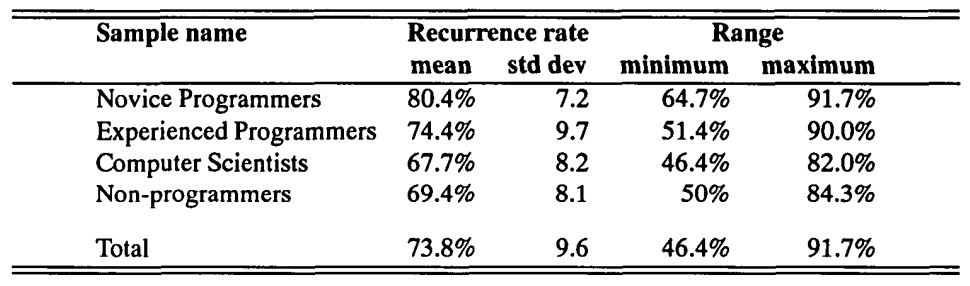
\includegraphics[width=\linewidth]{figures/greenberg/table_recurr-rate-in-different-samples.png}}
%   \caption{The average recurrence rate of the four sample UNIX user groups (Greenberg) \todotext{redo as an actual table}} 
% \end{figure}


\subsection{Maximum possible recalled characters}

\redtext{Recurrence rate represents how often people execute command line entries that were already entered before. Maximum possible recalled characters represents how many characters can be recalled from shell history assuming we store all previously entered commands. This metric show us the potential of shell history tools quantified in recalled characters.}

\todotext{TODO: Greenberg reports average command line entry length of 7.58 characters. Maximum possible recalled characters per command line submission was 4.43 characters. Whenever the user types in a new command line entry there can be no characters recalled; This lowers the maximum recalled characters per command line entry.}

\todotext{TODO: Our data shows average command line entry length of 29.26 characters. Maximum possible recalled characters per command line entry is 16.34 characters. We see a significant increase in the average command line entry compared to Greenberg. Naturally, this also increases the potential recalled characters.}

\redtext{This difference makes sense when we look at commands that are available today. There are new complex commands with subcommands and long options. Consider} \verb|git|\redtext{, it has many subcommands which accept different options; Additionally, the order of arguments matters.}

\todo{Is this where we talk about complex commands ??? }

\todotext{We conclude that the potential of shell history facilities has increased over the years because of differences in shell usage, available commands, and shell itself.}

\subsection{Maximum possible recalled characters including prefix matches}
% prefix matches

\todotext{TODO: We found situations in our collected shell history where the user gradually modified recently submitted command line entries. These entries often did not exactly match any of previous command lines entries but they were very similar. Workflows that repeat parts of previous command line entries are an opportunity for shell history use. Previously introduced metric does not account for this type of command line entry reuse. To estimate the potential of shell history tools we measured the potential recalled characters considering prefix matches.}

\todotext{TODO: Maximum possible recalled characters including prefix matches is 26.77 characters per command line entry. You can see that this is close to the average command line entry length; This means that almost all command line entries share prefixes of significant length with previously submitted command line entries. This of course does not mean that it is possible to create a shell history system that achieves these amounts of character reuse. However the potential of history facilities is great. }




\todo{NOTE: avg recurrence rate \& avg max possible recalled characters \%\%\%}
% ALL avg cmdline = 29.269552945461168
% >>> Avg recurrence rate = 70.29523637022278
% >>> Max avg recalled characters = 16.34658576344865
% >>> Max avg recalled characters (including prefix matches) = 26.770874841514217


% greenberg 1993 vs now
% the average length of command lines is 7.58
% recurrence rate is 74.4% for Experienced Programmers (avg group), max chars. recalled for an optimal conditioning method is 4.43 characters predicted per submission.

\blind

\subsection{Potential recalled characters as a function of distance}

\todotext{TODO: add graph with all subjects combined or separated}

\begin{figure}
\centering
  \tmpframe{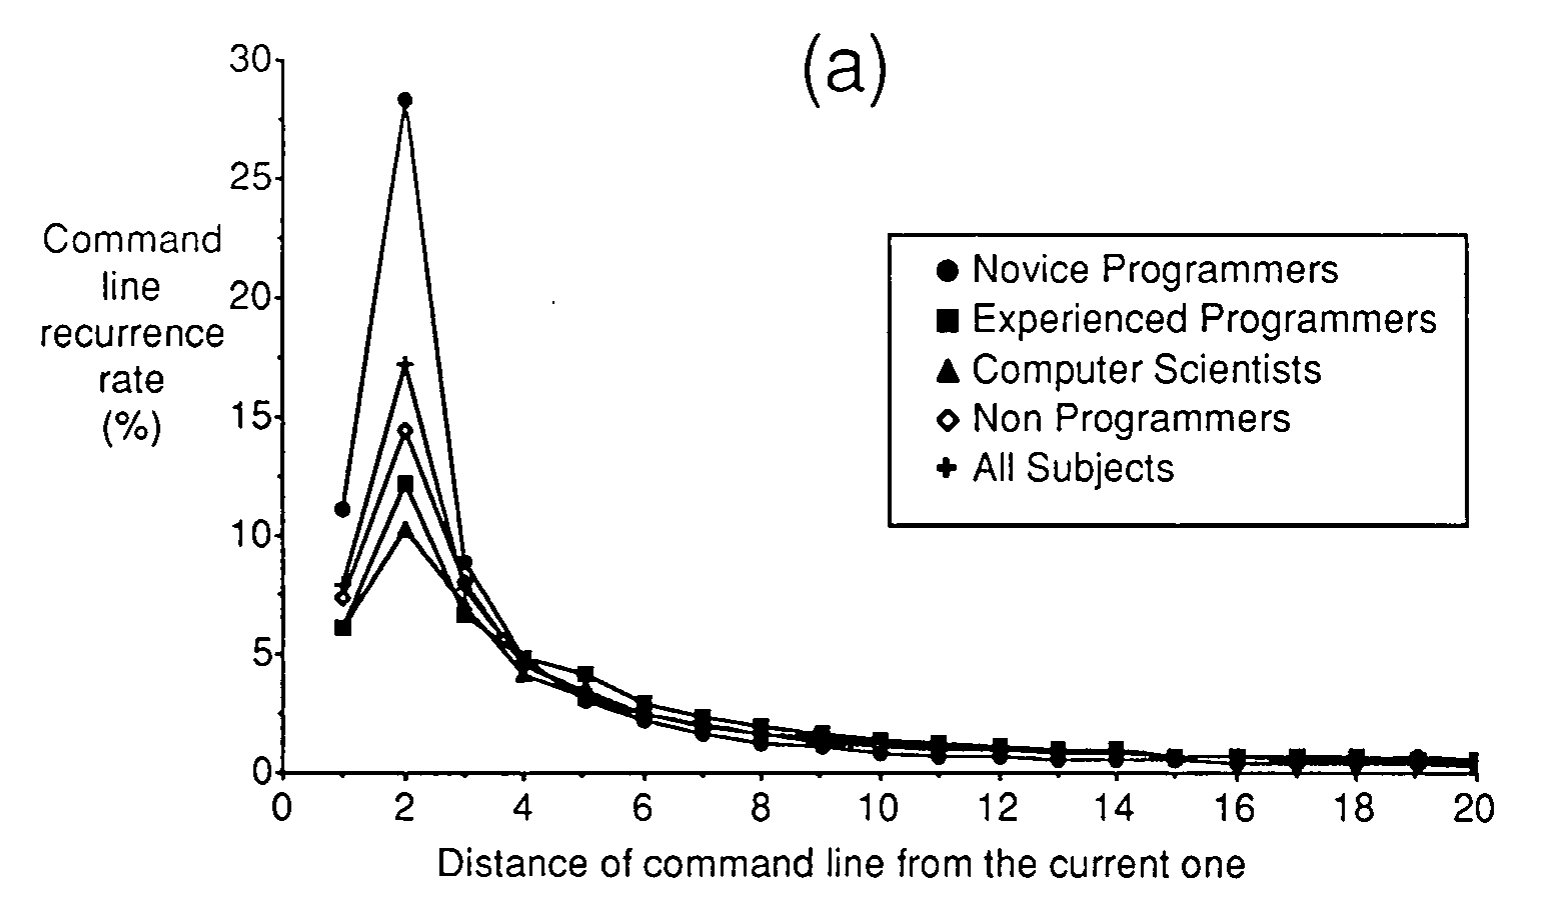
\includegraphics[width=\linewidth]{figures/greenberg/plot_ref_cmdline-recurr-rate.png}}
  \caption{Recurrence distribution as a measure of distance. (Greenberg)}
\end{figure}

\begin{figure}
\centering
  \tmpframe{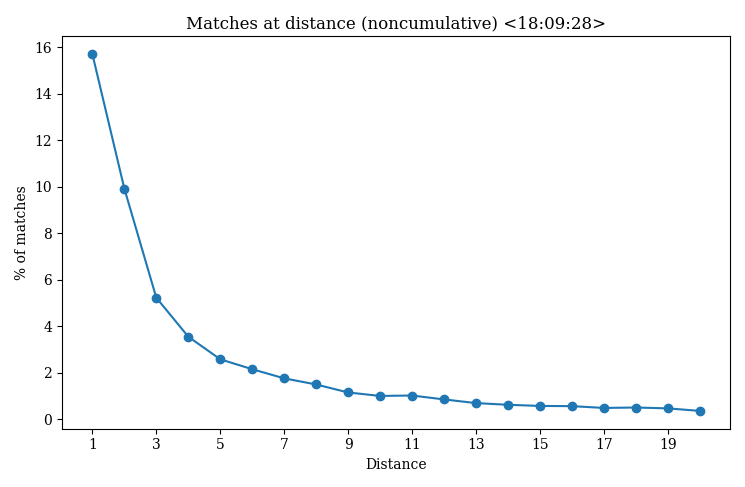
\includegraphics[width=\linewidth]{figures/greenberg_new/plot_cmdline-recurr-rate.png}} 
  \caption{Recurrence distribution as a measure of distance.}
\end{figure}


\subsection{Command line entry vocabulary}

\todotext{TODO: find out where to put this !!! }

\todo{!!! conclusions from plots !!!}



\todotext{}




% Figure 5.6. Command line vocabulary size vs. the number of commands entered for four typical individuals.

\begin{figure}
\centering
  \tmpframe{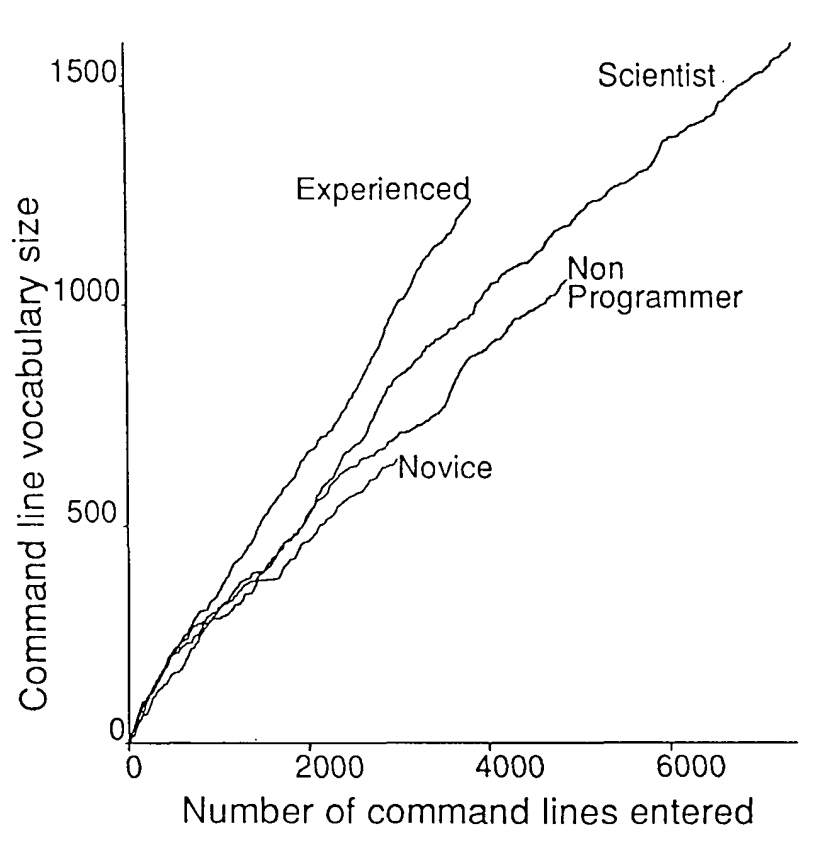
\includegraphics[width=0.6\linewidth]{figures/greenberg/plot_ref_cmdline-vocab-size.png}}
  \caption{Command line vocabulary size vs. the number of commands
entered for four typical individuals. (Greenberg)}
\end{figure}

\begin{figure}
  \tmpframe{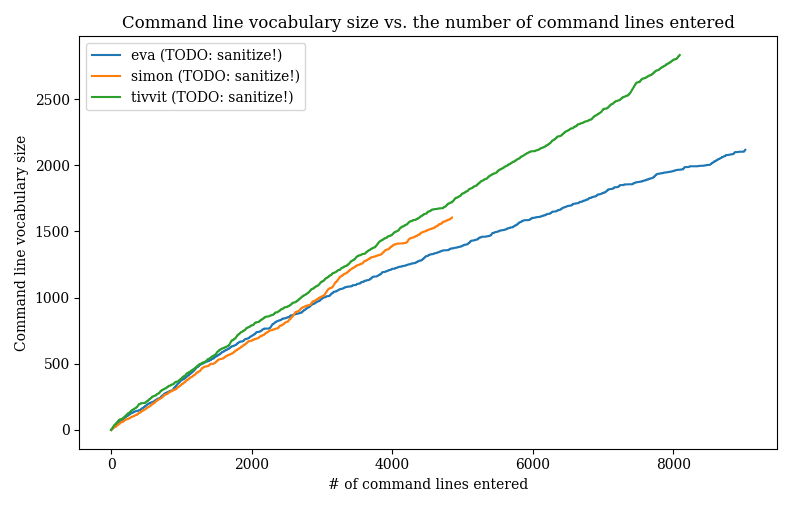
\includegraphics[width=\linewidth]{figures/greenberg_new/plot_cmdline-vocab-size.png}}
  \caption{Command line vocabulary size vs. the number of commands
entered for a single experienced programmer \todotext{TODO: title}}
\end{figure}

\subsection{Predicting command lines entered by users}
\todotext{TODO: Predicting users' next command line - what is the state of the art, what are the disadvantages}

\blind[2]


\todotext{How have shell usage changed since standard shell history features and greenberg study - longer commands, more commands; sessions (there can be more terminal windows open -> history is not strictly sequential anymore); }



\blind[3]


\section{How people use shell history}

\todo{DESC: practical chapter with concrete examples based on the standard history features}

In the previous sections, we have looked at existing research about shell usage. We compared the findings from literature with a small sample of data we collected ourselves. 

We saw that there is a lot of recurrence and patterns in the way people use shell. These properties of shell usage show us the potential of shell history. When designing any shell history tools we should leverage and respect them.

However, we should not blindly assume that leveraging the recurrence and patterns of shell usage will produce useful history tools. To see the full picture, we need to examine not only how people use shell but how they use shell history.  

For example, studying your shell usage could show us that you often use a specific command line entry. However, there is a significant difference in workflow based on whether you prefer to recall the entry from history or if you prefer to type it out. A shell history mechanism that suggests command line entries that you never retrieve from history provides zero value. 

Consider another example; You download and install a new history tool that is supposed to increase your productivity. It promises to predict what command line entry you are going to use next. It is activated when you press \verb|arrow_up|. There is an issue with such a tool; You are likely used to having access to recent history entries when you press \verb|arrow_up|. You probably have a strong expectation that \verb|arrow_up| gives you previous history entry; Chances are that sometimes you press \verb|arrow_up| and execute the retrieved history entry without even reading it. History tool that breaks this expectation will cause mistakes and ultimately you will be forced to either change your habits or uninstall the tool.  

\todotext{TODO: no usable research on how people use shell facilities (Greenberg has usage from csh with history expansion only)}
\todotext{TODO: to get an idea of how people use shell history we explored and "initiated/participated" in online discourse}
\blind 


\subsection{Online discourse about shell history}

\todotext{TODO: talk about our online research - my twitter thread, hackernews threads, SO questions, etc.}

\todotext{SO and SE show the standard issues, questions, wanted features}
\todotext{TW thread shown things people use and features they want}


\todotext{TODO: Naturally, people are selective about what they share online this skews the available information. People are not likely to share the basic usage habits they do not even realize they have. BUT they will share their custom configurations and scripts. }
% We find mentions of issues they run into when using standard history features.

\subsection{Common shell history issues and usage patterns}

\todotext{TODO: In this section, we present our observations and highlight sentiments that people voice online. Our observations include issues people face when using shell history, what people expect from shell history and }

\todotext{TODO: We focus on more general findings. We leave specific tools people use for a later section.}


\subsubsection*{Robustness of standard shell history}

The most common issues people ask questions about are related to robustness of the history.

People expect shell history to gracefully handle multiple \textbf{simultaneous sessions}. This is not the case; The user can run into multiple issues depending on what is the default configuration in the package provided by the distribution.
\todotext{The most common issue is - losing history from sessions because the last session overwrites the history file. Some people expect the history to be shared between sessions and it is nontrivial to set it up (in bash, zsh has an option)}
\todotext{The most severe issue is a race condition that can cause bash to lose the entire shell history. There is no mechanism that ensures that two shell sessions will not write out shell history at the same time. People have reported losing their whole history because of this issue. When users shutdown their machine with multiple open terminals the chance of the race condition increases because all the shell sessions will be "killed" by the "system" at roughly the same time.}


\todotext{Unlimited history - people expect}
\todotext{unlimited search}


\todotext{Full transcript - people expect}


\subsubsection*{Basic/Standard shell history features/usage}

\subsubsection*{Contextual history}

\subsubsection*{Control over what gets into history}

\subsubsection*{Shell history across multiple devices / Synchronizing history between devices}

\subsubsection*{Smart shell history features}



\todotext{TODO: introduce personas - HERE?!}

\todotext{TODO: Experienced user}

\todotext{TODO: Novice shell user}



\todotext{TODO: describe "use cases" - HERE?! - yes because we want to compare the standard history features to our solution in the end using these use cases }

\todotext{USECASE: fix a typo in a previous command - press arrow up, }

\todotext{USECASE: use: sudo !! to run a previous command with sudo}

\todotext{USECASE: recall a recent command - press arrow up 5-6 (3-8) times; type prefix + press arrow up 2-3 times NOTE: recent in time vs. recent in command sequence}

\todotext{USECASE: come back to a project and continue previous work on it}

\todotext{USECASE: find a long (w/ many arguments/options) curl request to github api}

\todotext{USECASE: run a recent git command}

\todotext{USECASE: find a command using datetime, command(first word) }

\todotext{USECASE: use case where we find something in history and want to find a similar command immediately: 1 use resh cli to find the first command, 2 execute, 3 arrow\_up, 4 ctrlR gives you similar results to what you found before}

\todo{TODO: Provide a concrete example for all of the use cases !}

\blind[4]

\todotext{TODO: conclusion of the chapter}

\blind

\section{Existing history tools and common history configurations}
\todo{chapter with various possible solutions, inspirations, etc.}

\todotext{TODO: mention our online research again}
\todotext{TODO: shell history configurations options}


\subsection{how much do people configure and customize \redtext{TODO: better title?}} 
\todotext{TODO: Some people enjoy actively tweaking and customizing their setups and we look at the configurations they are sharing to explore possible features and options. - the lesson here is to keep things extensible and hackable.}

\todotext{TODO: Large group of people does not want to spend time configuring and customizing their shell and expect it to just work.}
\todotext{TODO: There is one major reason and one minor reason. The major reason is that to customize and configure you need to either pause whatever you are doing or dedicate some extra time for it. This seems obvious but the fact that customization is extra work will deter many people from configuring their shells. }
\todotext{TODO: The lesson here is that the default configuration should provide good out of the box experience for the average user. }

\todotext{TODO: Another reason people avoid customization is when they often ssh to many different machines. The issue is that they get used to the custom the local environment and then they miss the customizations on different machines they visit. Depending on how much time they spend on other machines, it might be more convenient to just use the standard defaults everywhere.}

\todotext{TODO: This kind of issue is tough one to deal with; People may be hesitant to even use new history tools because of this issue. We should be aware of this issue and consider how could shell history work across multiple devices.}

\todotext{TODO: common configuration options and what problems are they solving}

\todotext{-$>$ issues caused by running simultaneous sessions - SO full of questions, semi tricky config, PROMPT-COMMAND, histappend option }

\todotext{TODO: per directory history}

\todotext{TODO: per date + session history}

\todotext{TODO: more configurations ...}

\todotext{TODO: configuration management projects e.g.: oh-my-zsh}

\todotext{TODO: many people avoid custom configuration because they move between many devices (ssh into servers)}

\subsection{Existing history tools \todotext{TODO: split into more subsections}}

\todotext{TODO: fuzzy search - fzf}

\todotext{TODO: hstr - addresses the issue of Ctrl-R that only shows one result}

\begin{figure}
  \tmpframe{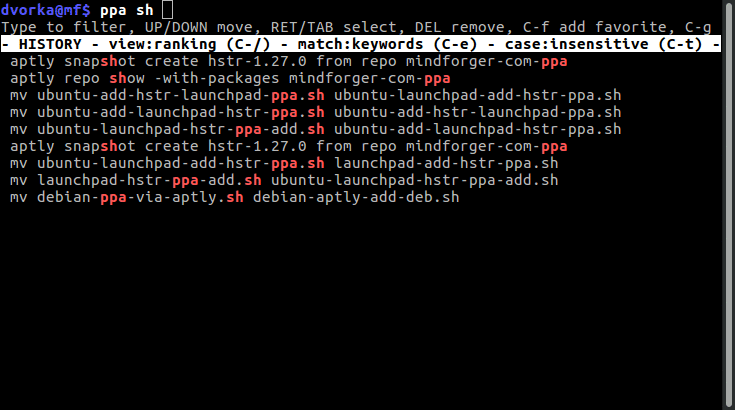
\includegraphics[width=\linewidth]{figures/misc/hstr-v2-30.png}}
  \caption{Hstr screenshot \todotext{TODO: title}}
\end{figure}

\todotext{TODO: bashhub - contextual cloud shell history}

\todotext{TODO: mcfly - contextual NN powered history search}

\todotext{TODO: advanced-shell-history - contextual history with smart querying - too buggy to be useful}


\todotext{TODO: Other less notable shell history tools - underdeveloped, non-interactive, ...}


\subsection{History features of Read-eval-print loops}

\todotext{TODO: Python - arrow down}

\subsection{History features of Friendly interactive shell}

\todotext{TODO: autosuggestions}

\todotext{TODO: contextual autosuggestions}

\todotext{TODO: missing reverse search}


\blind[4]

\todotext{TODO: short conclusion about history tools, configurations, etc.}



\section{Available contextual information}

\todotext{TODO: intro}

\subsection{Directly available contextual information}

\blind[2]

\subsection{Derivable contextual information}

\blind[2]

\subsection{Usage of history features as a context}

\blind[2]

\todotext{TODO: conclusion of the section}



\chapter{Design}
\todotext{TODO: intro describe contents of the chapter}

\blind
\todo{order of design chapters can change}
\section{Recording contextual history}

\todotext{TODO: what to record}

\blind[2]

\section{Interactive history features} % front-end

\todotext{TODO: intro}

\blind

\subsection{Standard history features}

\todotext{TODO: describe why it's important to respect the standard history features}

\todotext{TODO: which history features are we keeping/enhancing/leaving intact}

\blind[3]

\todotext{TODO: conclusion for further design ?}



\subsection{Core ideas, principals, design decisions, and features}\todo{weird title}

\todotext{TODO: intro: ideas in this chapter are essential for this work / project}

\todotext{TODO: features of the project - weird todo}

\blind[3]

\subsection{Possible features}

\todotext{TODO: intro: this section describes features that were considered during the design - for each feature we evaluate how well it would fit with the rest of the design. Some of the features were explicitly suggested by users and some features are included for the sake of completeness (because they make sense).}

\todo{TODO: list the features}


\section{Back-end}\todo{I don't like the title}

\blind

\section{Testing the design}

\todotext{TODO: explain why we want to test the design - intro}

\todotext{TODO: principals, guidelines, etc. are we are using}

\blind[3]

\chapter{Implementation}
\todo{merge sections to have less of them}
\todotext{describe layout/contents of the chapter}

\blind

\section{Daemon}\todo{do we need this or is introduction enough}

\blind

\section{Choosing Go}

\blind[3]

\section{Recording shell history with context}

\blind

\subsection{History format}

\todotext{NOTE: both on disk and in transfer}

\blind

\subsection{Shell integration and hooks}

\blind

\subsection{History record merging}

\blind

\section{Custom arrow key bindings}

\todotext{TODO: intro: we want arrow key bindings to be able to record usage related metadata + it's a good idea to have the option to customize and use context to enhance arrow key bindings. Plus impossibility of gathering usage data and using the default bindings (at least in Bash)}

\blind

\subsection{Keybinding custom functions in zsh}

\blind

\subsection{Keybinding custom functions in Bash}

\blind

\subsection{Reverting keybindings}

\blind

\subsection{Universal keybinding library}
\todotext{TODO: explain why: as you see Bash and zsh have a different ways of supporting custom keybindings. To simplify our codebase we extracted the keybind setting logic into a library. (unified way to set keybindings)}

\blind

\subsection{Performance issues of custom keybindings in Bash}

\blind


\section{Fullscreen command line history searching application}

\todo{TODO: subsections}


\section{Daemon components}

\todotext{TODO: describe why we need components}

\begin{figure}
  \tmpframe{\includegraphics[width=\linewidth]{figures/daemon-components.jpg}}
  \caption{One image. \todotext{TODO: write a title}}
  \label{fig:TODO}
\end{figure}

\subsection{Server}

\subsection{History file}

\subsection{Session history}
\todotext{TODO: explain: there are implications for the daemon if we want responsive arrow key bindings}

\subsection{Expired session tracking}


\subsection{Signal handling}

\blind

\section{Control and configuration}

\blind

\section{Installation, updates, and build process}

\todotext{TODO: explain how simple the installation is. plus updates.}

\blind

\subsection{Installation and updates}
\todotext{TODO: explain how installation works}

\blind

\subsection{Production and development build process}
\todotext{TODO: explain the build process}

\blind[2]


\chapter{Testing and Evaluation}

\todotext{TODO: describe layout/contents of the chapter}

\todotext{TODO: describe how history tools can be usable}

\todotext{TODO: describe what influences usability of the tools}

\todotext{TODO: explain which parts of the system should be tested and why}

\blind[3]

\section{Metrics}

\todotext{TODO: describe why we use metrics}

\subsection{Metrics traditionally used to evaluate history tools}\todo{break down into more subsections ?}

\todotext{TODO: describe which metrics were used for history tools in the past}

\subsection{Newly suggested metrics}\todo{break down into more subsections ?}

\todotext{TODO: suggest new metrics + explain how they are better than the original ones}

\subsection{Evaluation using suggested metrics}

\todotext{TODO: explain used methods}

\todotext{TODO: use metrics to evaluate usefulness of the work}


\section{Use cases}

\todotext{TODO: we rolled out the prefix search as a default and we received zero negative feedback. Study of usage of history utilities does indicate that prefix search does not interfere with normal arrow up workflow. We asked users about the feature and some of them were not aware of it.}


\begin{conclusion}

\todotext{TODO: rewrite conclusion}

I have analysed shell history features available in current shells. I explored available history tools and found both positive and negative inspiration.

\par I have found previous research on how people use shell and shell history.  
I have collected a sample of shell history. I have analyzed the collected usage data and compared it to data used in existing research. I have found which characteristics of shell usage changed over time and which characteristics stayed the same. I have concluded that most of the principals and ideas from the existing research do still hold. I have found out that potential recalled characters increased 4 times since the study was conducted. This and other differences reinforced the idea that it makes sense to design and develop new history related tools. 

\par I have conducted a market research to find out how people interact with shell history and what are the workflows that are not well supported nowadays. I have modelled personas representing target users of the system. I have put together use cases based on actual shell history I have collected.
I have designed a contextual shell history tools based on problems and suggestions from existing literature, user-centered design guidelines and principals, information learned via market research, and modelled personas.
I have actively sought feedback from users during both design and implementation. 

I have used usability principals and heuristics to test and evaluate the design.

\par I have implemented a significant portion of the design. The project unobtrusively records shell history with context. It does both use context to offer relevant history records and for searching via fullscreen command line application.
I have made sure that it's easy to install, update, configure and use. I have shared the resulting implementation with community and received overwhelmingly positive feedback and interest of contributors. Project was downloaded and installed over 5 hundred times since January. Github page of the project consistently attracts daily visitors.  

\par I have described a number of possible metrics. I have explained why simple metrics are not sufficient. I have described the drawbacks of metrics in general. I have suggested meaningful metrics that can be used to evaluate shell history tools. I have used the suggested metrics to evaluate my implementation where possible. 

\par I have used modelled personas and use cases to evaluate utility and usability of the system.
I have used real life user data to evaluate user experience of the solution.


I have made it easier to collect and study usage of shell and shell history in future research.
I have proved that having contextual shell history brings many benefits. 
I have demonstrated public demand for history tools. 
I have created a universal shell library for binding custom functions to keys with the option to revert to previous state. 




\todotext{TODO: write future work}

\end{conclusion}

\bibliographystyle{iso690.bst}
\bibliography{ref}

\appendix

%\printglossaries

\chapter{Contents of SD card}\label{app:SDcontent}

\todotext{TODO: Visualise the contents of enclosed media. Use of dirtree is recommended. Note that directories src and text with appropriate contents are mandatory.}


\begin{figure}
	\dirtree{%
		.1 readme.txt\DTcomment{the file with CD contents description}.
		.1 data\DTcomment{the data files directory}.
		.2 graphs\DTcomment{the directory of graphs of experiments}.
		.3 *.eps\DTcomment{the B/W graphs}.
		.3 *.png\DTcomment{the color graphs}.
		.3 *.dat\DTcomment{the graphs data files}.
		.1 exe\DTcomment{the directory with executable WBDCM program}.
		.2 wbdcm\DTcomment{the WBDCM program executable (UNIX)}.
		.2 wbdcm.exe\DTcomment{the WBDCM program executable (Windows)}.
		.1 src\DTcomment{the directory of source codes}.
		.2 wbdcm\DTcomment{the directory of WBDCM program}.
		.3 Makefile\DTcomment{the makefile of WBDCM program (UNIX)}.
		.2 thesis\DTcomment{the directory of \LaTeX{} source codes of the thesis}.
		.3 figures\DTcomment{the thesis figures directory}.
		.3 *.tex\DTcomment{the \LaTeX{} source code files of the thesis}.
		.1 text\DTcomment{the thesis text directory}.
		.2 thesis.pdf\DTcomment{the Diploma thesis in PDF format}.
		.2 thesis.ps\DTcomment{the Diploma thesis in PS format}.
	}
\end{figure}


\end{document}
